We discuss the architecture and the three applications. BY modifing the error function, we can change the performance, give an example with anisotropic or systematic error.

SciKit-SurgeryFRED implements a simple user interface \ref{fig:surgery_fred}, to demonstrate registration of a pre-operative image to intra-operative space. At startup a target is placed at a random location within the pre-operative image, shown as a red circle. The standard deviation of the \gls{FLE} is randomly sampled from a uniform distribution 
between 0.5 and 5.0 pixels \footnote{All units are in pixels, as the concepts being explored do not depend on the units used. Figure \ref{fig:surgery_fred} shows a brain MRI 458x512 pixels, by design SciKit-SurgeryFRED should work with other images of arbitrary dimensions.}. By default the \gls{FLE} is modelled as an isotropic (in 3 dimensions), normally distributed, and independent random variable, though this can be easiliy changed. The variance of the \gls{FLE} is shown at the top left (as expected value), along with number of number of fiducial markers. 

Clicking either image adds a fiducial marker to both images. The marker is added to the pre-operative image with no \gls{FLE}. \gls{FLE} is added to the marker location in the intra-operative image, visualised as the misalignment between the green circle centre and the crosshair. Once sufficent markers are placed ($>2$) the two sets of markers are registered as per \cite{Arun1987}. The expected values (variance) of the \gls{FRE} and \gls{TRE} are calculated 
as per \cite{Fitzpatrick1998}. The registration and statistical algorihms are implemented in SciKit-SurgeryCore \cite{matt_clarkson_2020_3965731}.

\cite{matt_clarkson_2020_3965731}

\begin{figure}
	\begin{center}
	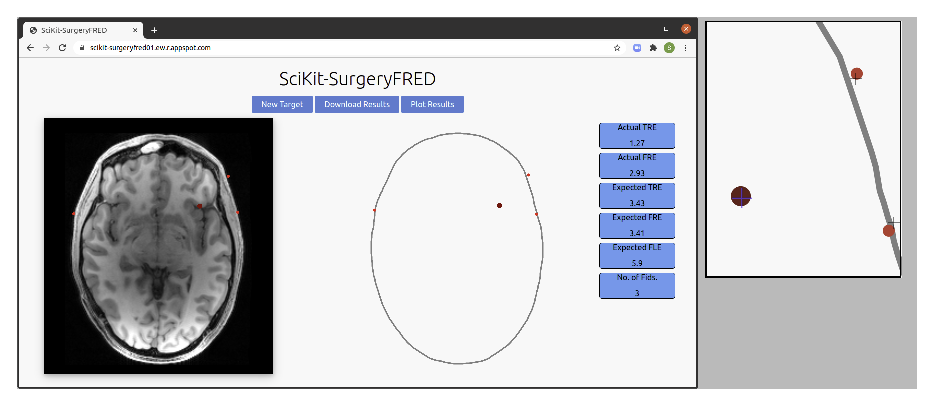
\includegraphics[width=0.9\linewidth]{scikit-surgeryfred_gui.eps}
		\caption{\label{fig:surgery_fred}SciKit-SurgeryFRED graphical user interface after 3 fiducials placed. The red sphere in the pre-operative image (left) represents a clinical target, which is located in the
		intra-operative space (middle) by fiducial based registration, using the fiducial markers (green). FLEis added to each marker in the intra-operative image, this is more clearly visible on the zoomed in images at the right. The resulting registration results in a TRE, shown by the misalignment of the red circle and crosshair 
		on the enlarged image at right. TRE and other statistics are shown across the top
		of the window.}
	\end{center}
\end{figure}


\subsection{Configuration of FLE}
